\documentclass[10pt]{article}
\usepackage{graphicx}
\usepackage{subcaption}
\usepackage[T1]{fontenc}
\usepackage{amsmath}
\usepackage{lipsum}
\usepackage{amsfonts}
\usepackage{hyperref}
\usepackage{mathtools}
\providecommand\given{}
\usepackage[utf8]{inputenc}
\usepackage[letterpaper,margin=1in]{geometry}
\usepackage[parfill]{parskip}
\usepackage[europeanresistors, american]{circuitikz}
\usetikzlibrary{arrows,shapes,calc,positioning}
\usetikzlibrary{shapes}
\usetikzlibrary{plotmarks}
\usepackage{tikz}
\usepackage{pgfplots}
\usepackage{xparse}
\usetikzlibrary{decorations.markings,positioning}
\definecolor{whitesmoke}{rgb}{0.90, 0.90, 0.90}
\definecolor{lightgray}{rgb}{0.73, 0.73, 0.73}% overrides default?
\definecolor{dimgray}{rgb}{0.51, 0.51, 0.51}
\pgfplotsset{compat=newest}
\usepgfplotslibrary{units}
\newcommand{\oscope}[2] % #1 = name , #2 = rotation angle
{
    \draw[thick,rotate=#2] (#1) circle (12pt)
    (#1) ++(-0.35,-0.1) -- ++(0.3,0.3) --++(0,-0.3)-- ++(0.3,0.3) --++(0,-0.3);
}
\def\therefore{\boldsymbol{\text{ }
\leavevmode
\lower0.4ex\hbox{$\cdot$}
\kern-.5em\raise0.7ex\hbox{$\cdot$}
\kern-0.55em\lower0.4ex\hbox{$\cdot$}
\thinspace\text{ }}}

\vspace{-8ex}
\date{}
\begin{document}

\title{\textbf{\Large{\textsc{ECE320:} Fields and Waves}} \\ \Large{Lab 3 Report: Design of a Double Stub Matching Network} \\ \textbf{\small{PRA106}}\vspace{-0.3cm}}
\author{Alp Tarım, Pranshu Malik \\ \footnotesize{1003860128}, \footnotesize{1004138916}\vspace{-3cm}}

\maketitle

\section{Introduction}

This laboratory session was focused on investigating the input impedance and reflection coefficient at the load, and
making transformations to the load impedance using a double stub network such that we are able to match the input impedance 
to the characteristic impedance of the transmission line. We also measured the voltage standing wave ratio (VSWR) for the 
same matching network to characterize its bandwidth. Figure 1 shows the schematic for a double-stub tuner and its equivalent 
circuit. Our theoretical work and measurements are based on the unknown \underline{"orange"} labelled load given to us. 

\vspace{-0.3cm}
\begin{figure}[h]
  \centering
  \begin{circuitikz}
    \draw
    (0,2) to [esource, l_=$\text{VNA}$] (0, 0) -- (2,0)
    to [tline, o-o] (4,0)
    to [tline, *-o] (6,0)
    to [tline, o-*] (8,0) -- (8.5,0)
    to [R, l_=$Z_L$] (8.5, 2) -- (8,2)
    to [tline, l=${d_0}$,*-o] (6,2)
    to [tline, o-o, l=${d_1}$] (4,2)
    to [tline, l=${Z_0, \beta, L}$, *-o] (2,2)
    to [R, l_=${Z_\text{VNA}=Z_0}$] (0, 2);

    \draw[thick] (6,2) -- (7, 0.5) -- (7,-1.5) -- (6,0);
    \draw[thick] (4,2) -- (5, 0.5) -- (5, -1.5) -- (4,0);
    \draw (0,0) to[short, *-*] node[ground]{} (0,0);
    \draw (6.2, -0.75) node{$L_1$} (6.2, -0.75);
    \draw (4.2, -0.75) node{$L_2$} (4.2, -0.75);
    \draw (5.75, 1) node{$Z_0, \beta$} (5.75, 1);
    \draw [dotted, thick] (4,-0.35) -- (4,2.35) (8,-0.35) -- (8,2.35);


    \draw
    (0,-2) to [esource, l_=$\text{VNA}$] (0, -4) -- (2,-4)
    to [tline, o-o] (4,-4)
    to [tline, *-o] (6,-4)
    to [tline, o-*] (8,-4) -- (8.5,-4)
    to [R, l_=$Z_L$] (8.5, -2) -- (8,-2)
    to [tline, l=${d_0}$,*-o] (6,-2)
    to [tline, o-o, l=${d_1}$] (4,-2)
    to [tline, l=${Z_0, \beta, L}$, *-o] (2,-2)
    to [R, l_=${Z_\text{VNA}=Z_0}$] (0, -2);

    \draw (0,-4) to[short, *-*] node[ground]{} (0,-4);
    \draw (4,-4) to [R, l=$jb_2$] (4,-2);
    \draw (6,-4) to [R, l=$jb_1$] (6,-2);
    \draw [dotted, thick] (4,-4.35) -- (4,-3.95) (4, -2.05) -- (4,-1.65) (8,-4.35) -- (8,-1.65);
  \end{circuitikz}
  \caption{A double-stub matching network with $d_0 = 3.4\text{ cm}$ and $d_1 = 3.8\text{ cm}$}
\end{figure}
\vspace{-0.4cm}

\section{Measurement of the Unknown Load Impedance}
The unknown load impedance was measured over a frequency range of $[300\text{MHz},1.3\text{GHz}]$, with and 
without de-embedding, using the VNA on a Smith Chart shown in Figure 2 (a) and (b). The values of the load 
impedance and admittance with its normalized form taking $Z_0=50\Omega$ are given in Table 1.

\begin{table}[h]
  \[
      \begin{array}{c|c}
          \textbf{Parameter} & \textbf{Value} \\ \hline
          Z_L & 31.08 + 9.32j \quad [\Omega]\\
          Y_L & 0.029 + 0.089j \quad [\Omega^{-1}]\\
          Z_\text{L,N} & 0.622 + 0.186j\\
          Y_\text{L,N} & 1.476 - 0.441j\vspace{-0.3cm}
      \end{array}
  \]
  \caption{Measured impedance and admittance of the unknown load}
\end{table}

Since there is an adapter and extension ports between the ends of the BNC cable and the load, they act as 
additional sections of transmission lines which cause a rotation of the impedance on the Smith chart, and 
we can undo this rotation by rotating (de-embedding) the measurement anti-clockwise (towards the load) by the same 
extension length. The lab aks to de-embed our load by $T = 0.2 \text{ ns}$ at $f=800\text{Mhz}$, which corresponds 
to a distance of $\frac{c\cdot T}{c/f} = (0.2\cdot10^{-9}\cdot 800\cdot 10^{6}) \lambda = 0.16\lambda \approx 6\text{ cm}$, 
where $\lambda$ is the wavelength of a wave propagating at the speed of light, $c$, with frequency $f$.

To de-embed the load we rotate $Z_\text{L,N}$ anti-clockwise (towards the load) by $0.16\lambda$ on the SWR circle, 
shown in Figure 2 (c), and we get $Z_\text{L,N}' = 0.85 - 0.45j$, which is coincidently very near $Y_\text{A,N}$ 
(see section 3), and corresponds to $Z_L' = 42.5 - 22.5j [\Omega]$, closely matching the result shown by the VNA 
in Figure 2 (b).

\begin{figure}[ht]
  \centering
  \begin{subfigure}[b]{0.45\textwidth}
      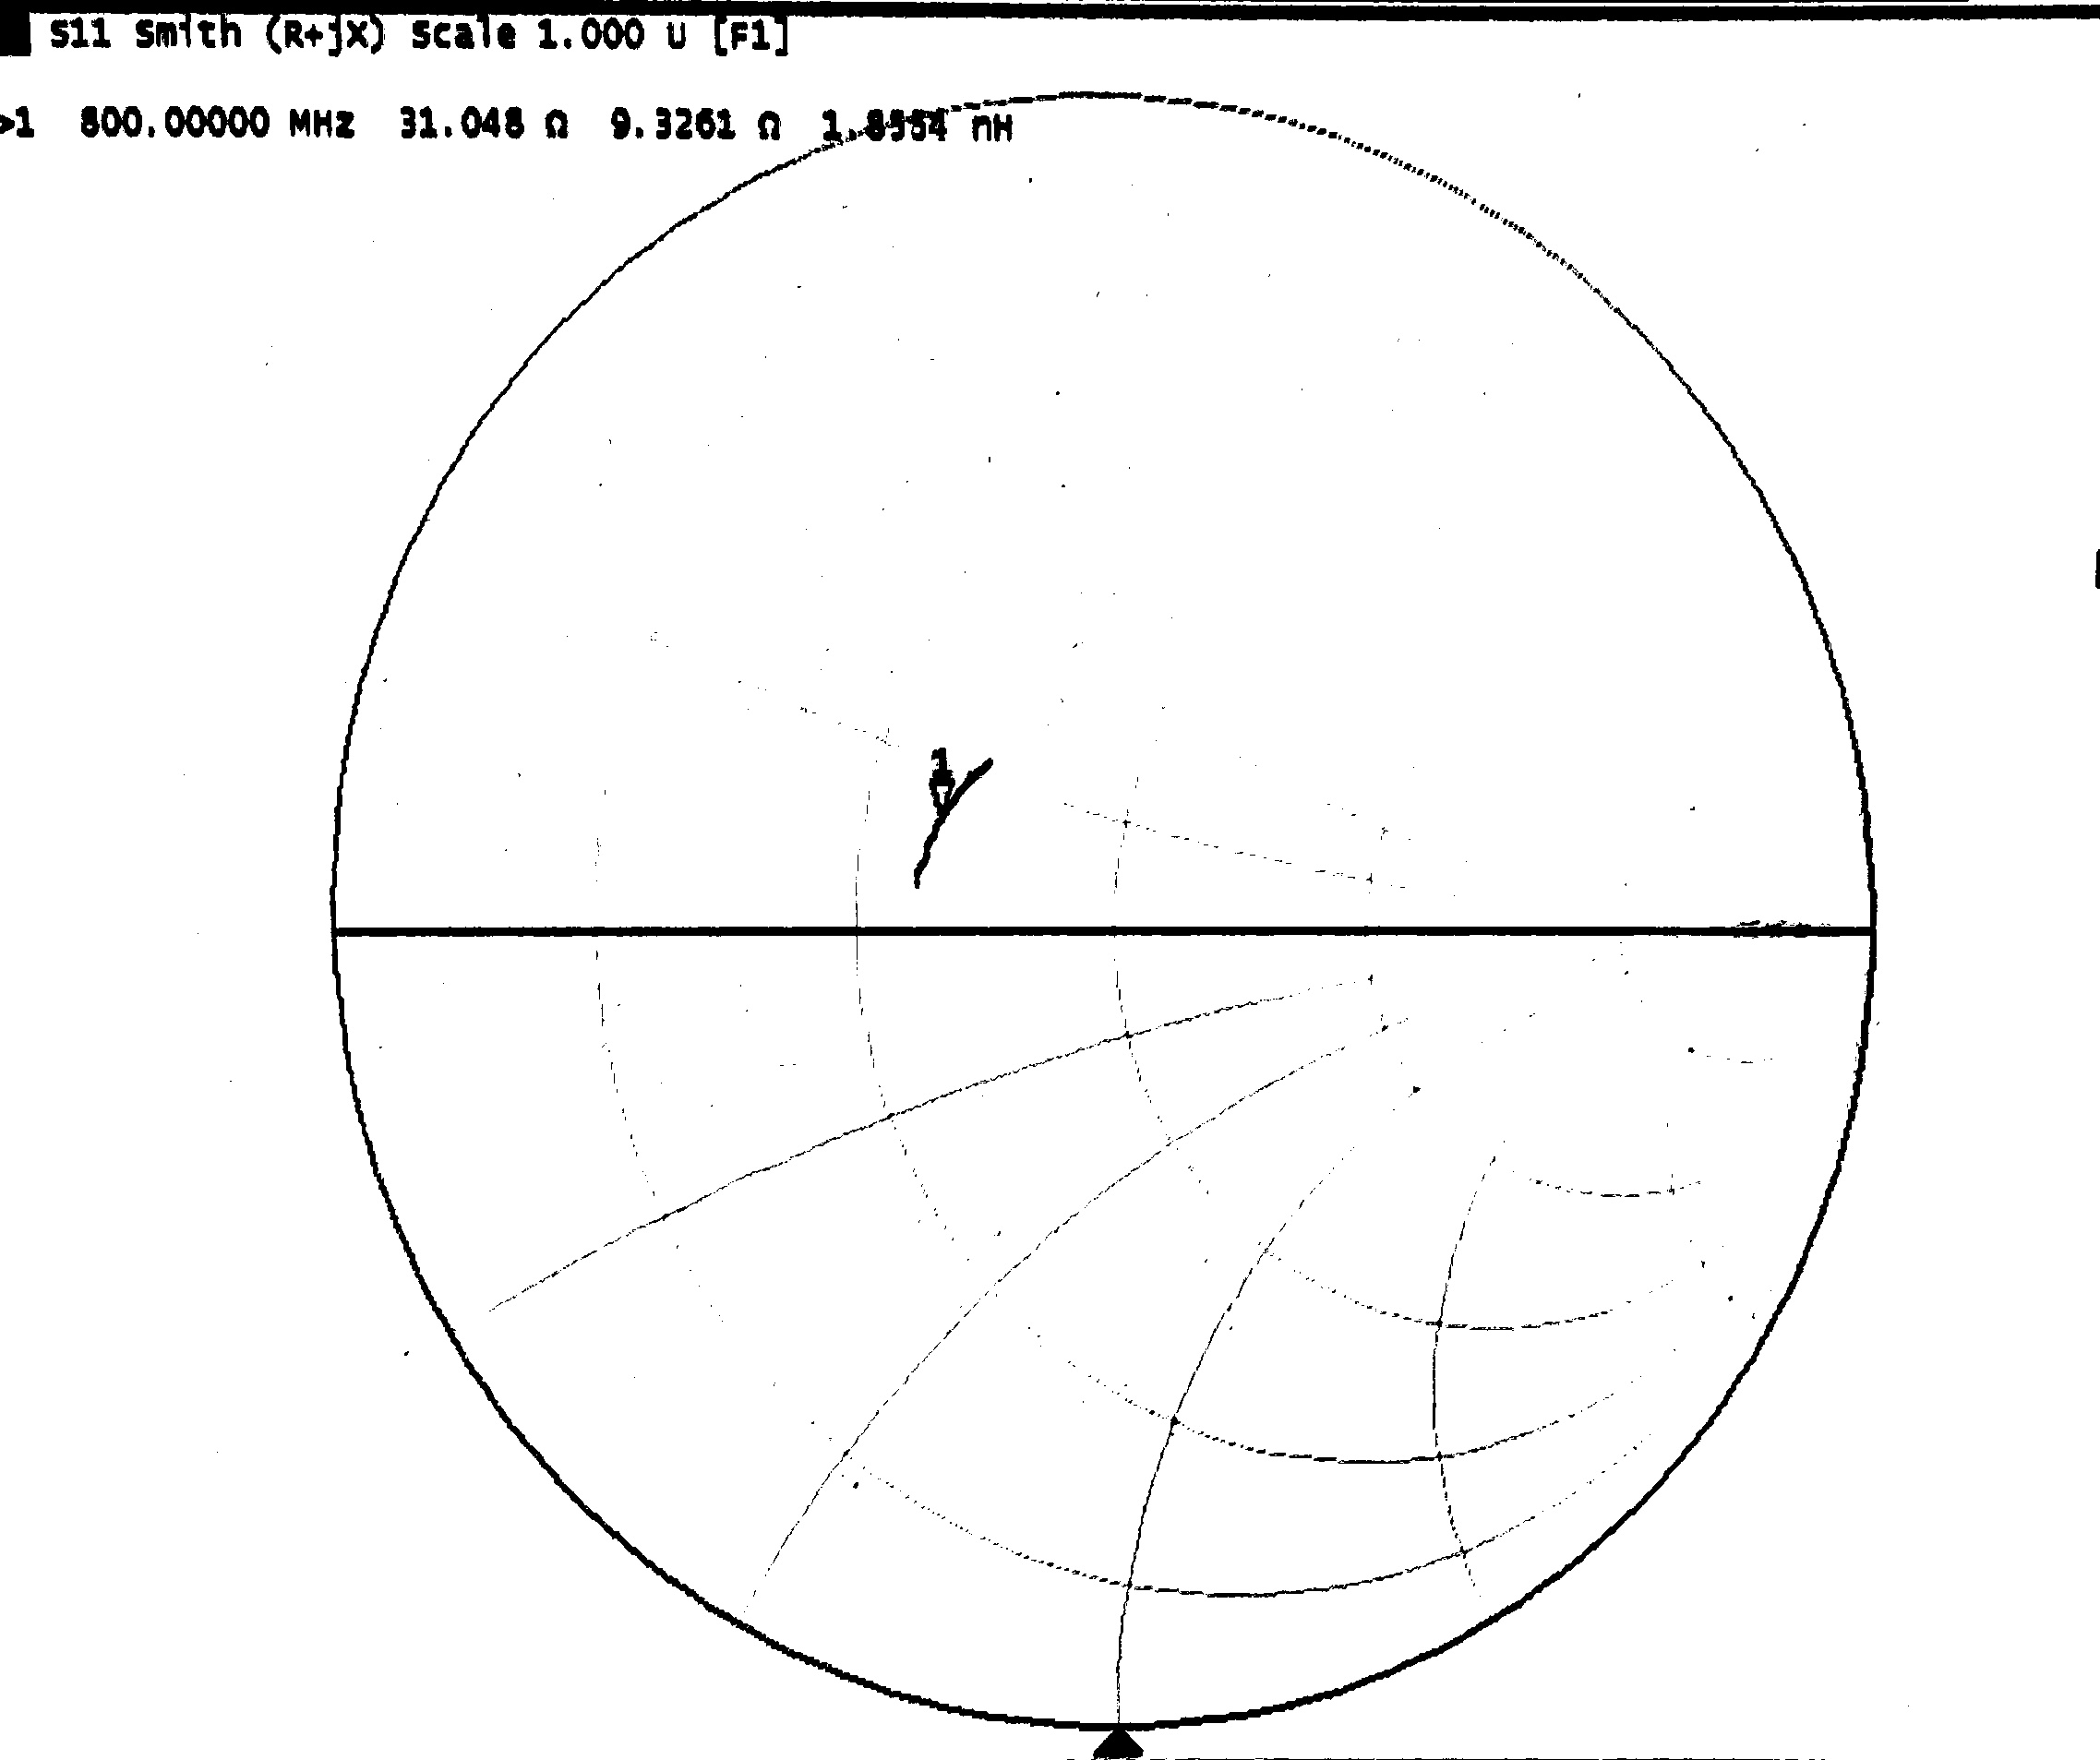
\includegraphics[width=\textwidth]{../photos/lab3/load_as_is.jpg}
      \caption{Measured impedance on the VNA}
  \end{subfigure}
  \quad
  \begin{subfigure}[b]{0.45\textwidth}
    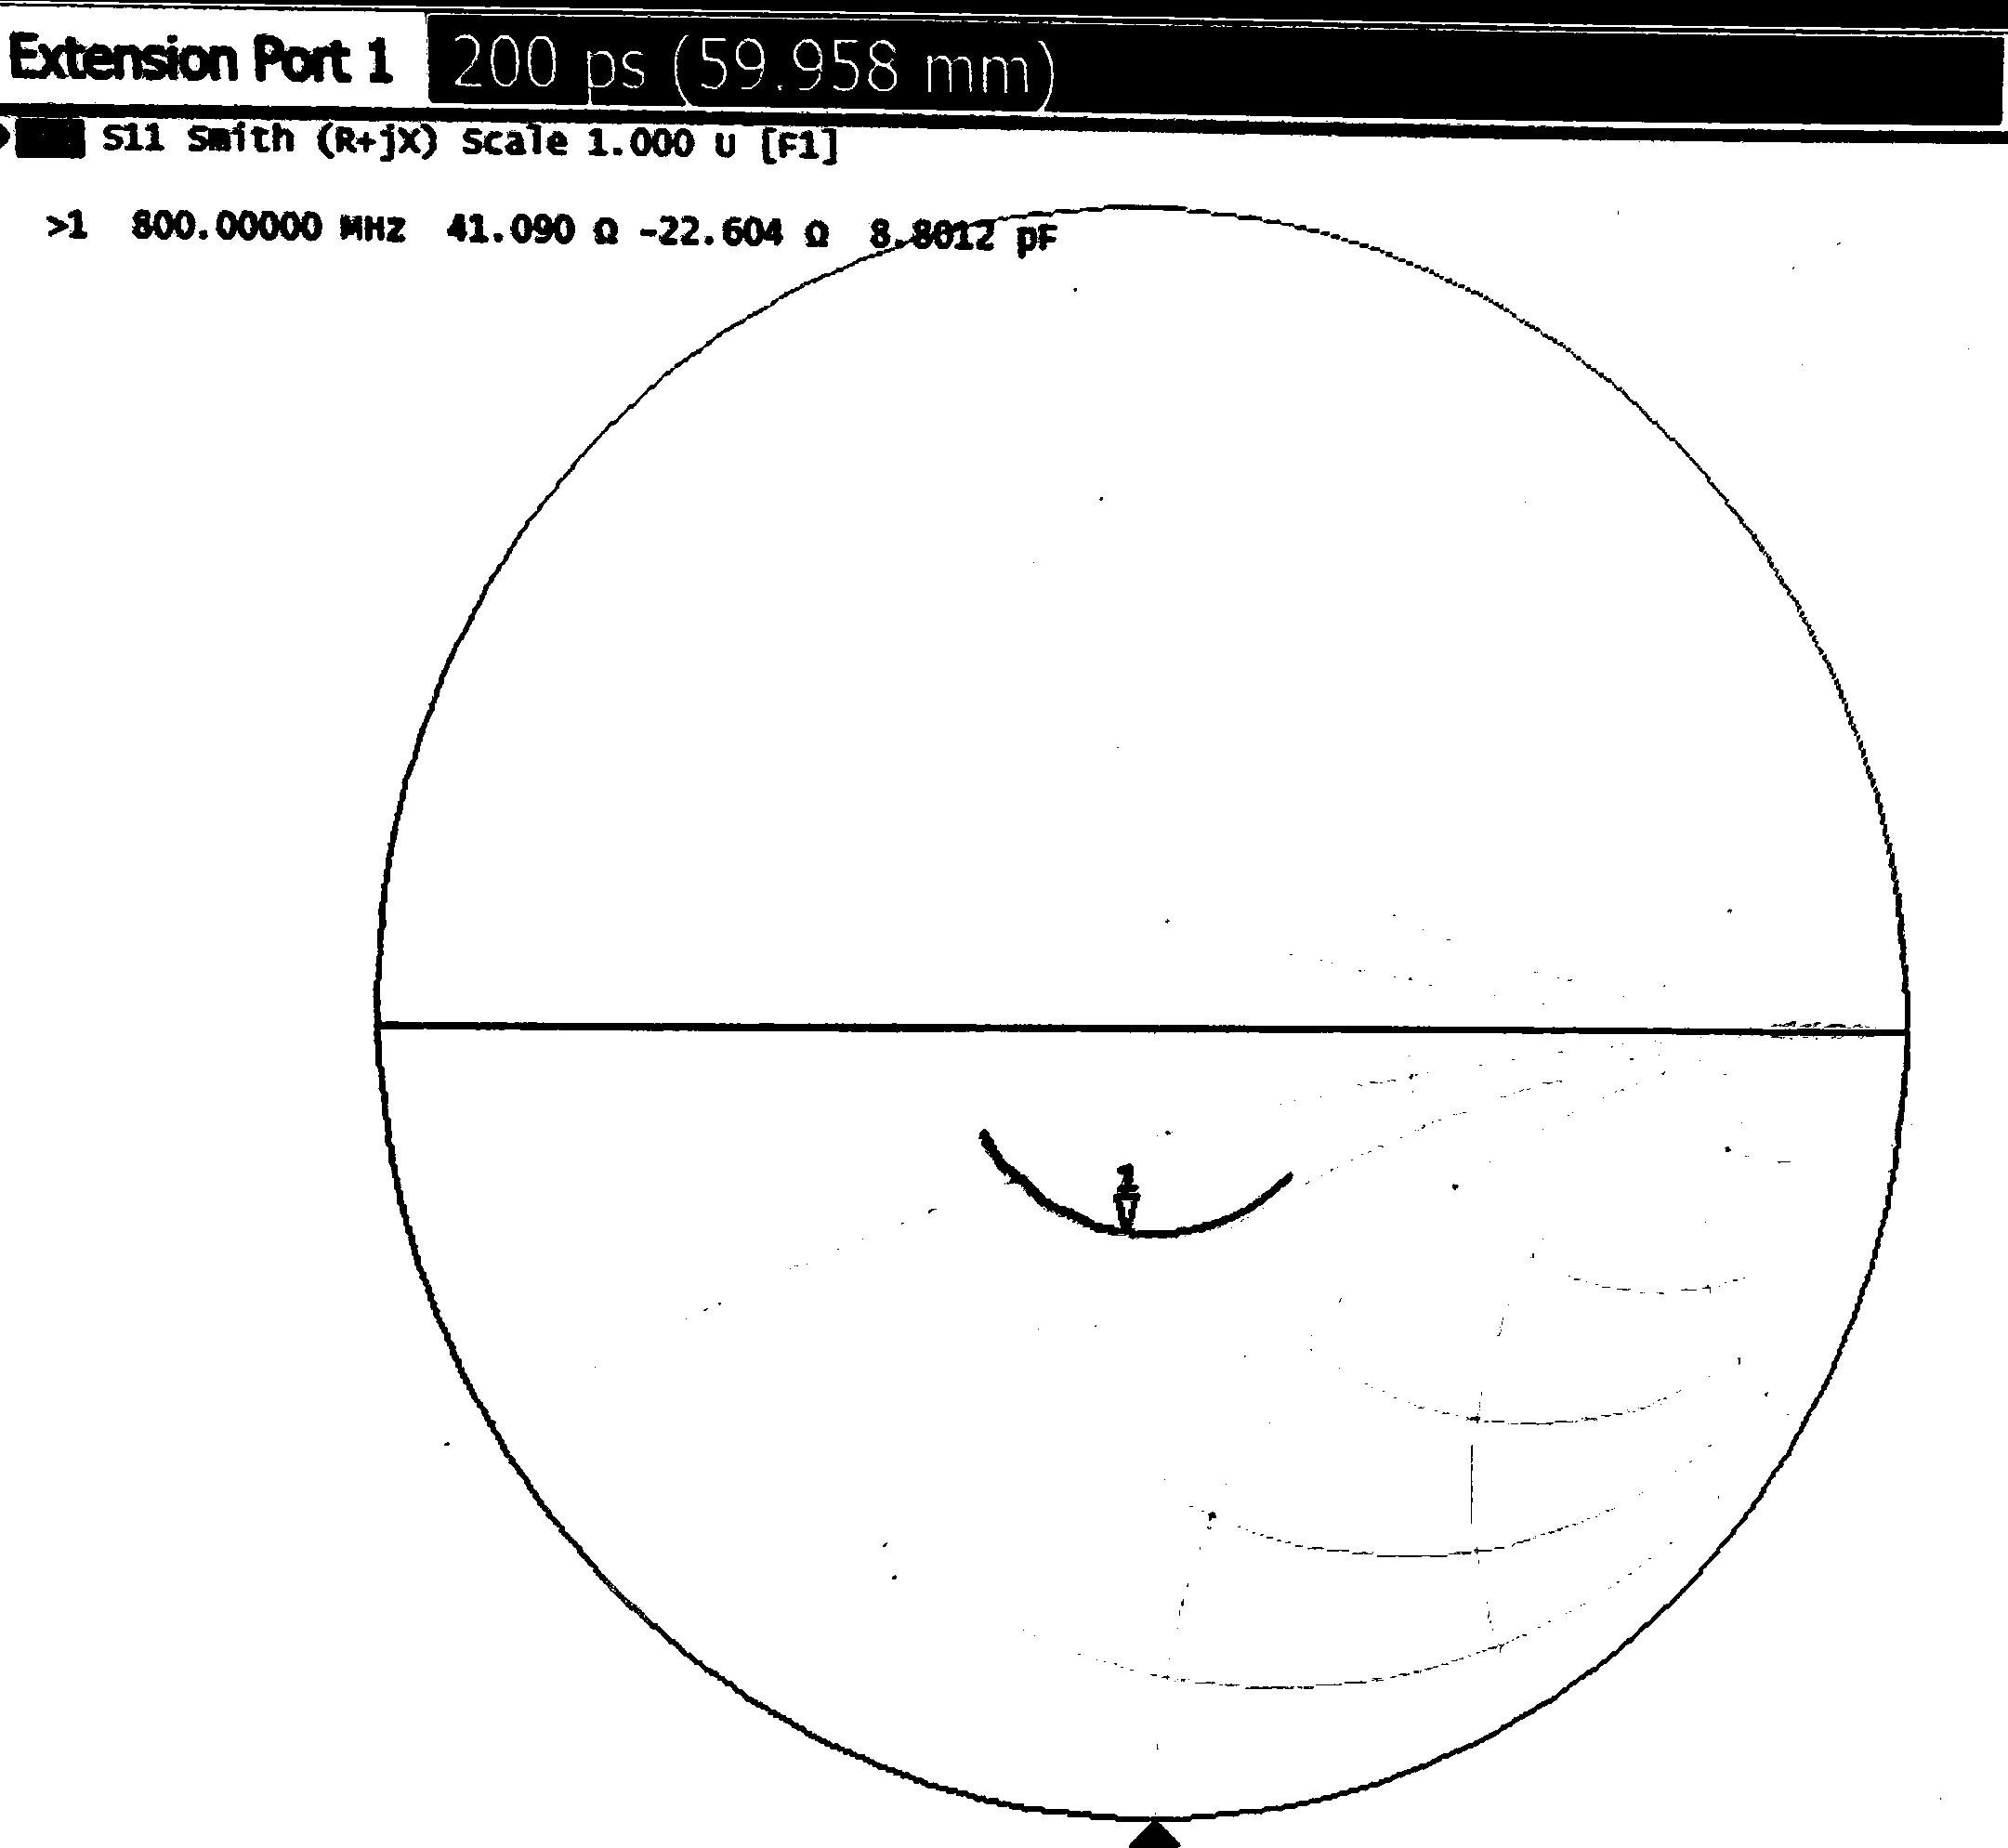
\includegraphics[width=\textwidth]{../photos/lab3/load_deembedded.jpg}
    \caption{Impedance de-embedded by $0.2\text{ ns}$ on the VNA}
  \end{subfigure}
  \begin{subfigure}[b]{0.37\textwidth}
    \begin{tikzpicture}
      \node[inner sep=0pt] (smith) at (0,0)
      {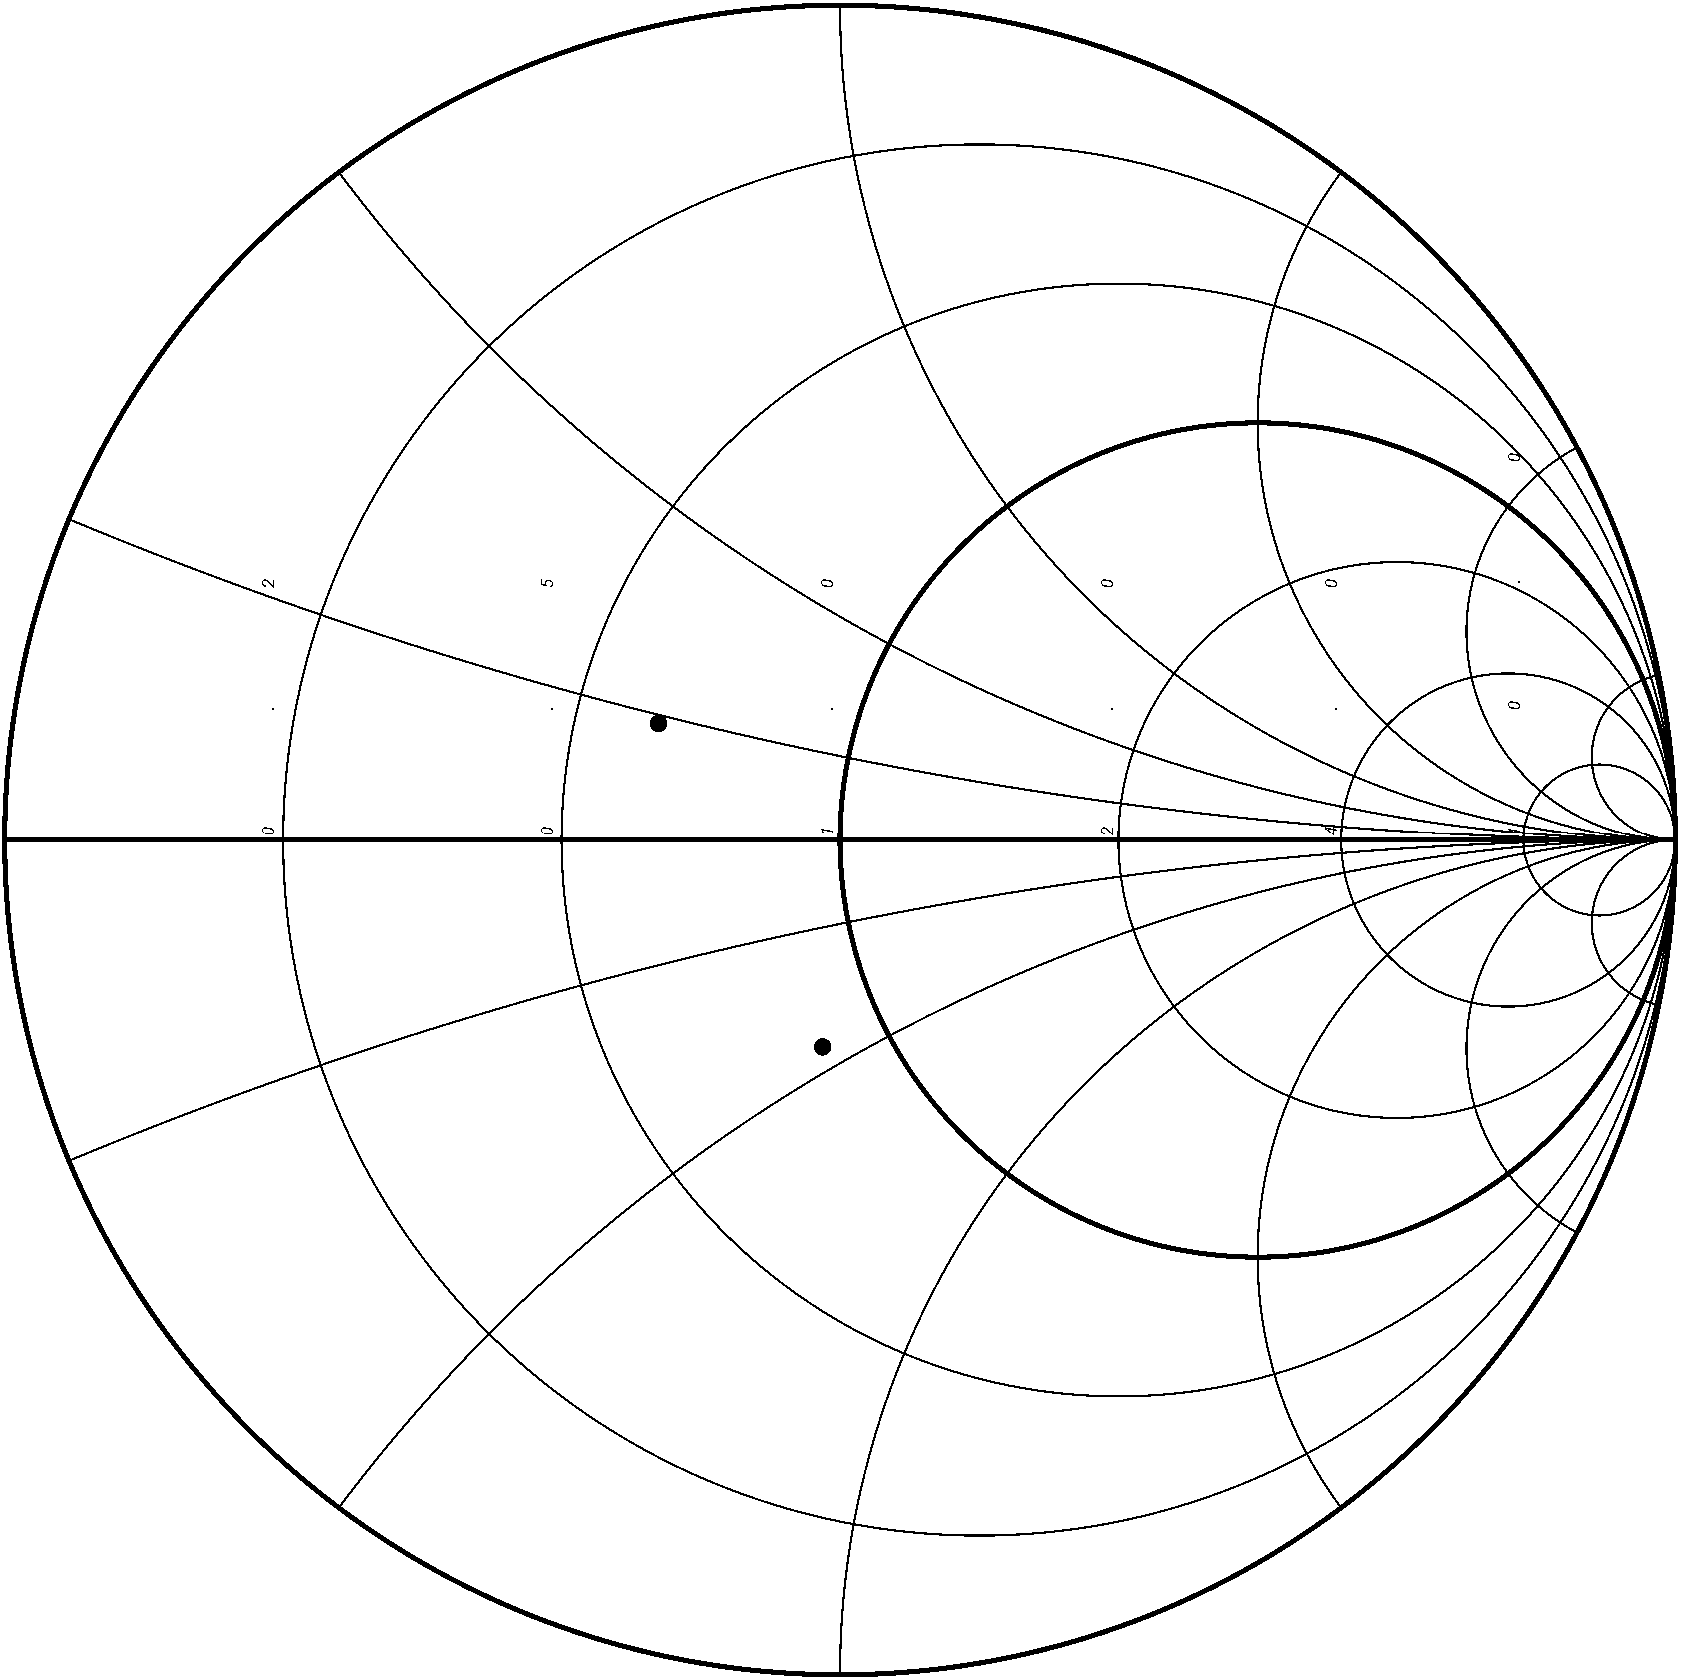
\includegraphics[width=\textwidth]{../photos/lab3/deembedding.png}};
      \node[draw, thick] at (-0.9,0.9) {$Z_\text{L,N}$};
      \node[draw, thick] at (0,-1.3) {$Z_\text{L,N}'$};
    \end{tikzpicture}
    \caption{Theoretically de-embedded impedance}
  \end{subfigure}
  \caption{Measured and de-embedded imepedance of the unknown load}
  \label{deembedding_load}
\end{figure}

\section{Designing a Double-stub Matching Network}

To start the matching process, we need to transform $Z_L$ by moving it towoards the generator by $d_0$ to reach the
first stub. The impedance at that loaction corresponds to rotating $Z_\text{L,N}$ by $0.09067\lambda$ clockwise on the 
SWR circle leading to $Z_\text{A,N} = 0.92 + 0.49j$, and $Y_\text{A,N} = 0.85 - 0.45j$ which was obtained by 
rotating $Z_\text{A,N}$ by $\frac{\lambda}{4}$ (or $\pi$ radians) on the same (SWR) circle. From here, we 
followed the double-stub matching procedure provided in the laboratory manual and the \underline{Smith charts and our 
calculations} for the lengths of both stubs are \underline{attached with this report}.

\begin{table}[h]
  \centering
  \begin{subtable}{0.8\textwidth}
    \[
      \begin{array}{c|c}
          \textbf{Fundamental Solution} & \textbf{Length in wavelengths}, \lambda \\ \hline
          \hat L_1 & 0.324 \lambda \\
          \hat L_2 & 0.210 \lambda \\
          \hat L_1' & 0.449 \lambda\\
          \hat L_2' & 0.445 \lambda\vspace{-0.25cm}
      \end{array}
  \]
  \caption{Calculated matching stub length pairs in wavelengths\vspace{0.15cm}}
  \end{subtable}
  \begin{subtable}{0.8\textwidth}
    \[
        \begin{array}{c|c}
            \textbf{Fundamental Solution} & \textbf{Length in} \text{ cm}\\ \hline
            L_1 & 12.15\\
            L_2 & 7.88\\
            L_1' & 16.84\\
            L_2' & 16.69\vspace{-0.25cm}
        \end{array}
    \]
    \caption{Calculated matching stub length pairs}
  \end{subtable}
\end{table}

The general solution in wavelengths for $n \in \mathbb{N} + \{0\}$ is, 
\begin{align*}
  \hat L_1 = 0.324 \lambda + \frac{n\lambda}{2} \quad &, \quad \hat L_2 = 0.210\lambda + \frac{n\lambda}{2}\\
  \hat L_1' = 0.449\lambda + \frac{n\lambda}{2} \quad &, \quad \hat L_2' = 0.445\lambda + \frac{n\lambda}{2}
\end{align*}
and the general solution in centimeters at $f = 800\text{ MHz}$ can be written as,
\begin{align*}
  L_1 = 12.15 + 18.75\cdot n \quad &, \quad L_2 = 7.88 + 18.75\cdot n\\
  L_1' = 16.84 + 18.75\cdot n \quad &, \quad L_2' = 16.69 +  18.75\cdot n
\end{align*}

\section{Experimental Measurement and Verification}

Our measurements were in close agreement with our theoretical calculations and can be found in Table 3. 
The measured values were within an error of $\pm2 \text{ cm}$ which is mainly due to the accumulation of error 
over a large number of operations done by hand on the Smith chart, and also due to the error in recording lengths 
of the stubs in the matching network. The Smith chart plots measured on the VNA can be found in Figure 3.

\begin{table}[h]
  \[
    \begin{array}{c|c}
        \textbf{Fundamental Solution} & \textbf{Length in} \text{ cm}\\ \hline
        L_1 &  10.5\\
        L_2 & 5.5\\
        L_1' & 17.1 \\
        L_2' & 16.8 \vspace{-0.25cm}
    \end{array}
\]
\caption{Experimentally measured stub lengths}
\end{table}

\begin{figure}[ht]
  \centering
  \begin{subfigure}[b]{0.45\textwidth}
      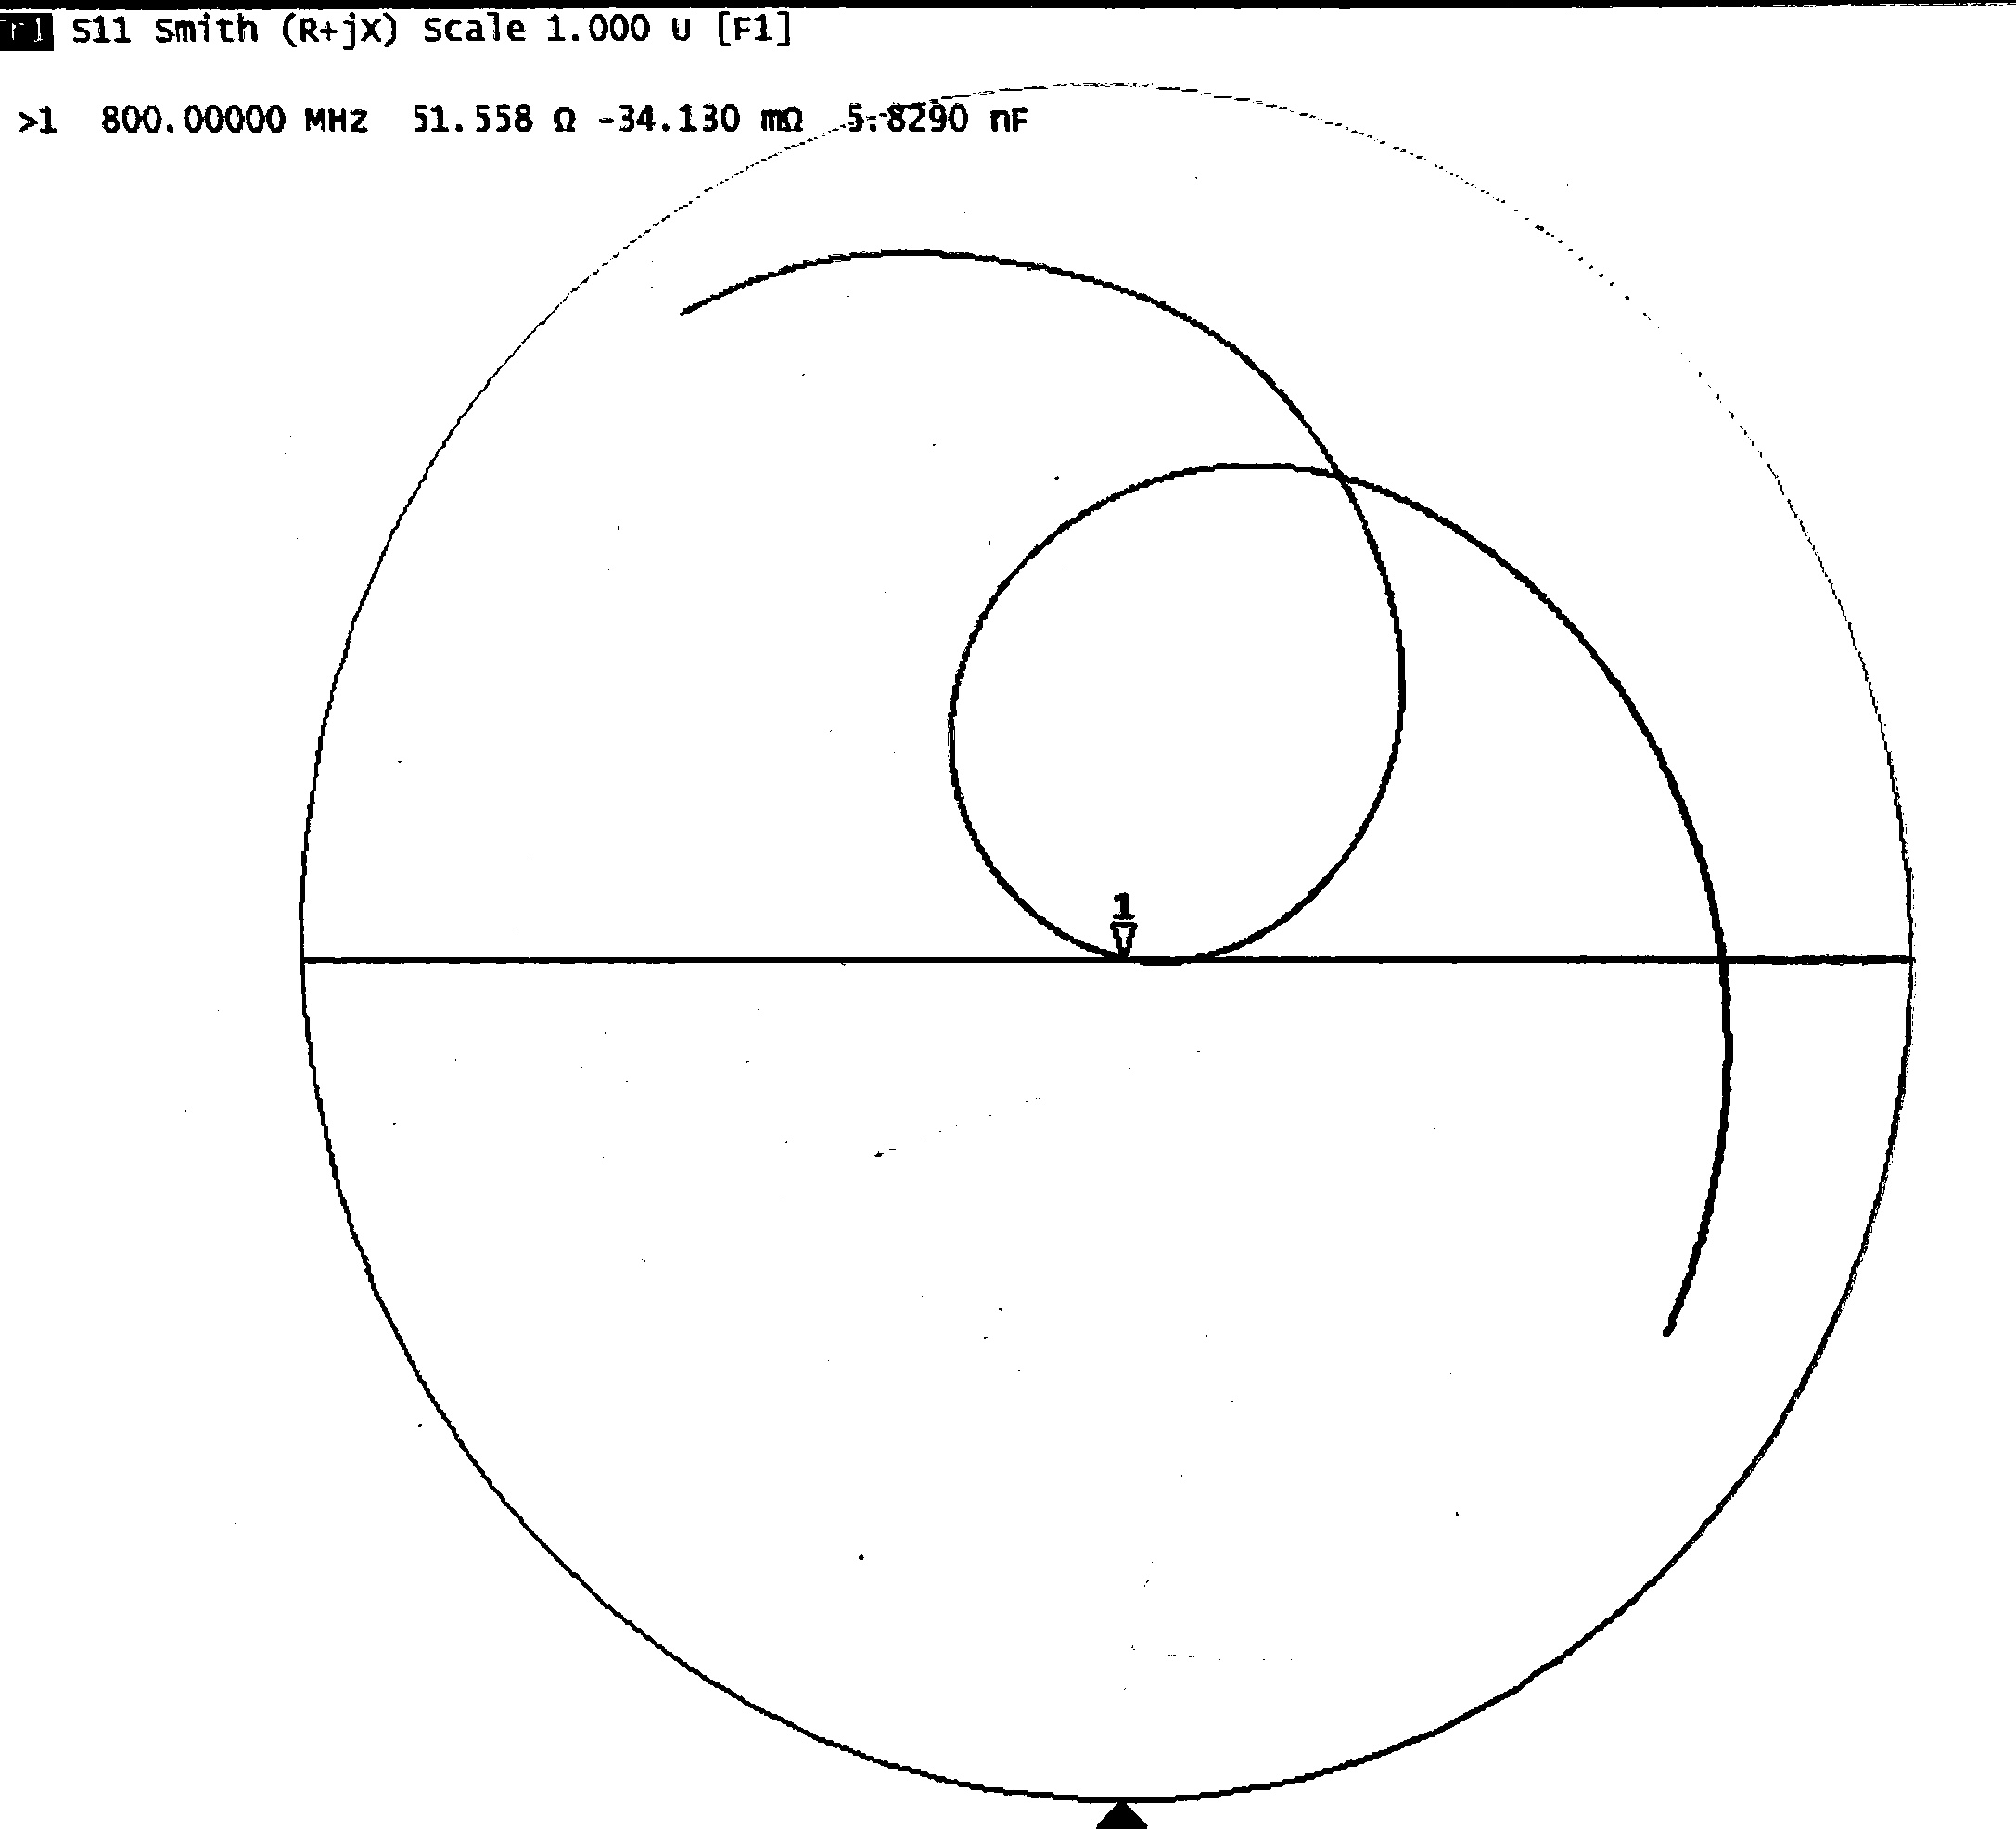
\includegraphics[width=\textwidth]{../photos/lab3/matching_short_pair.jpg}
      \caption{Matched load using the shorter length stubs}
  \end{subfigure}
  \quad
  \begin{subfigure}[b]{0.45\textwidth}
    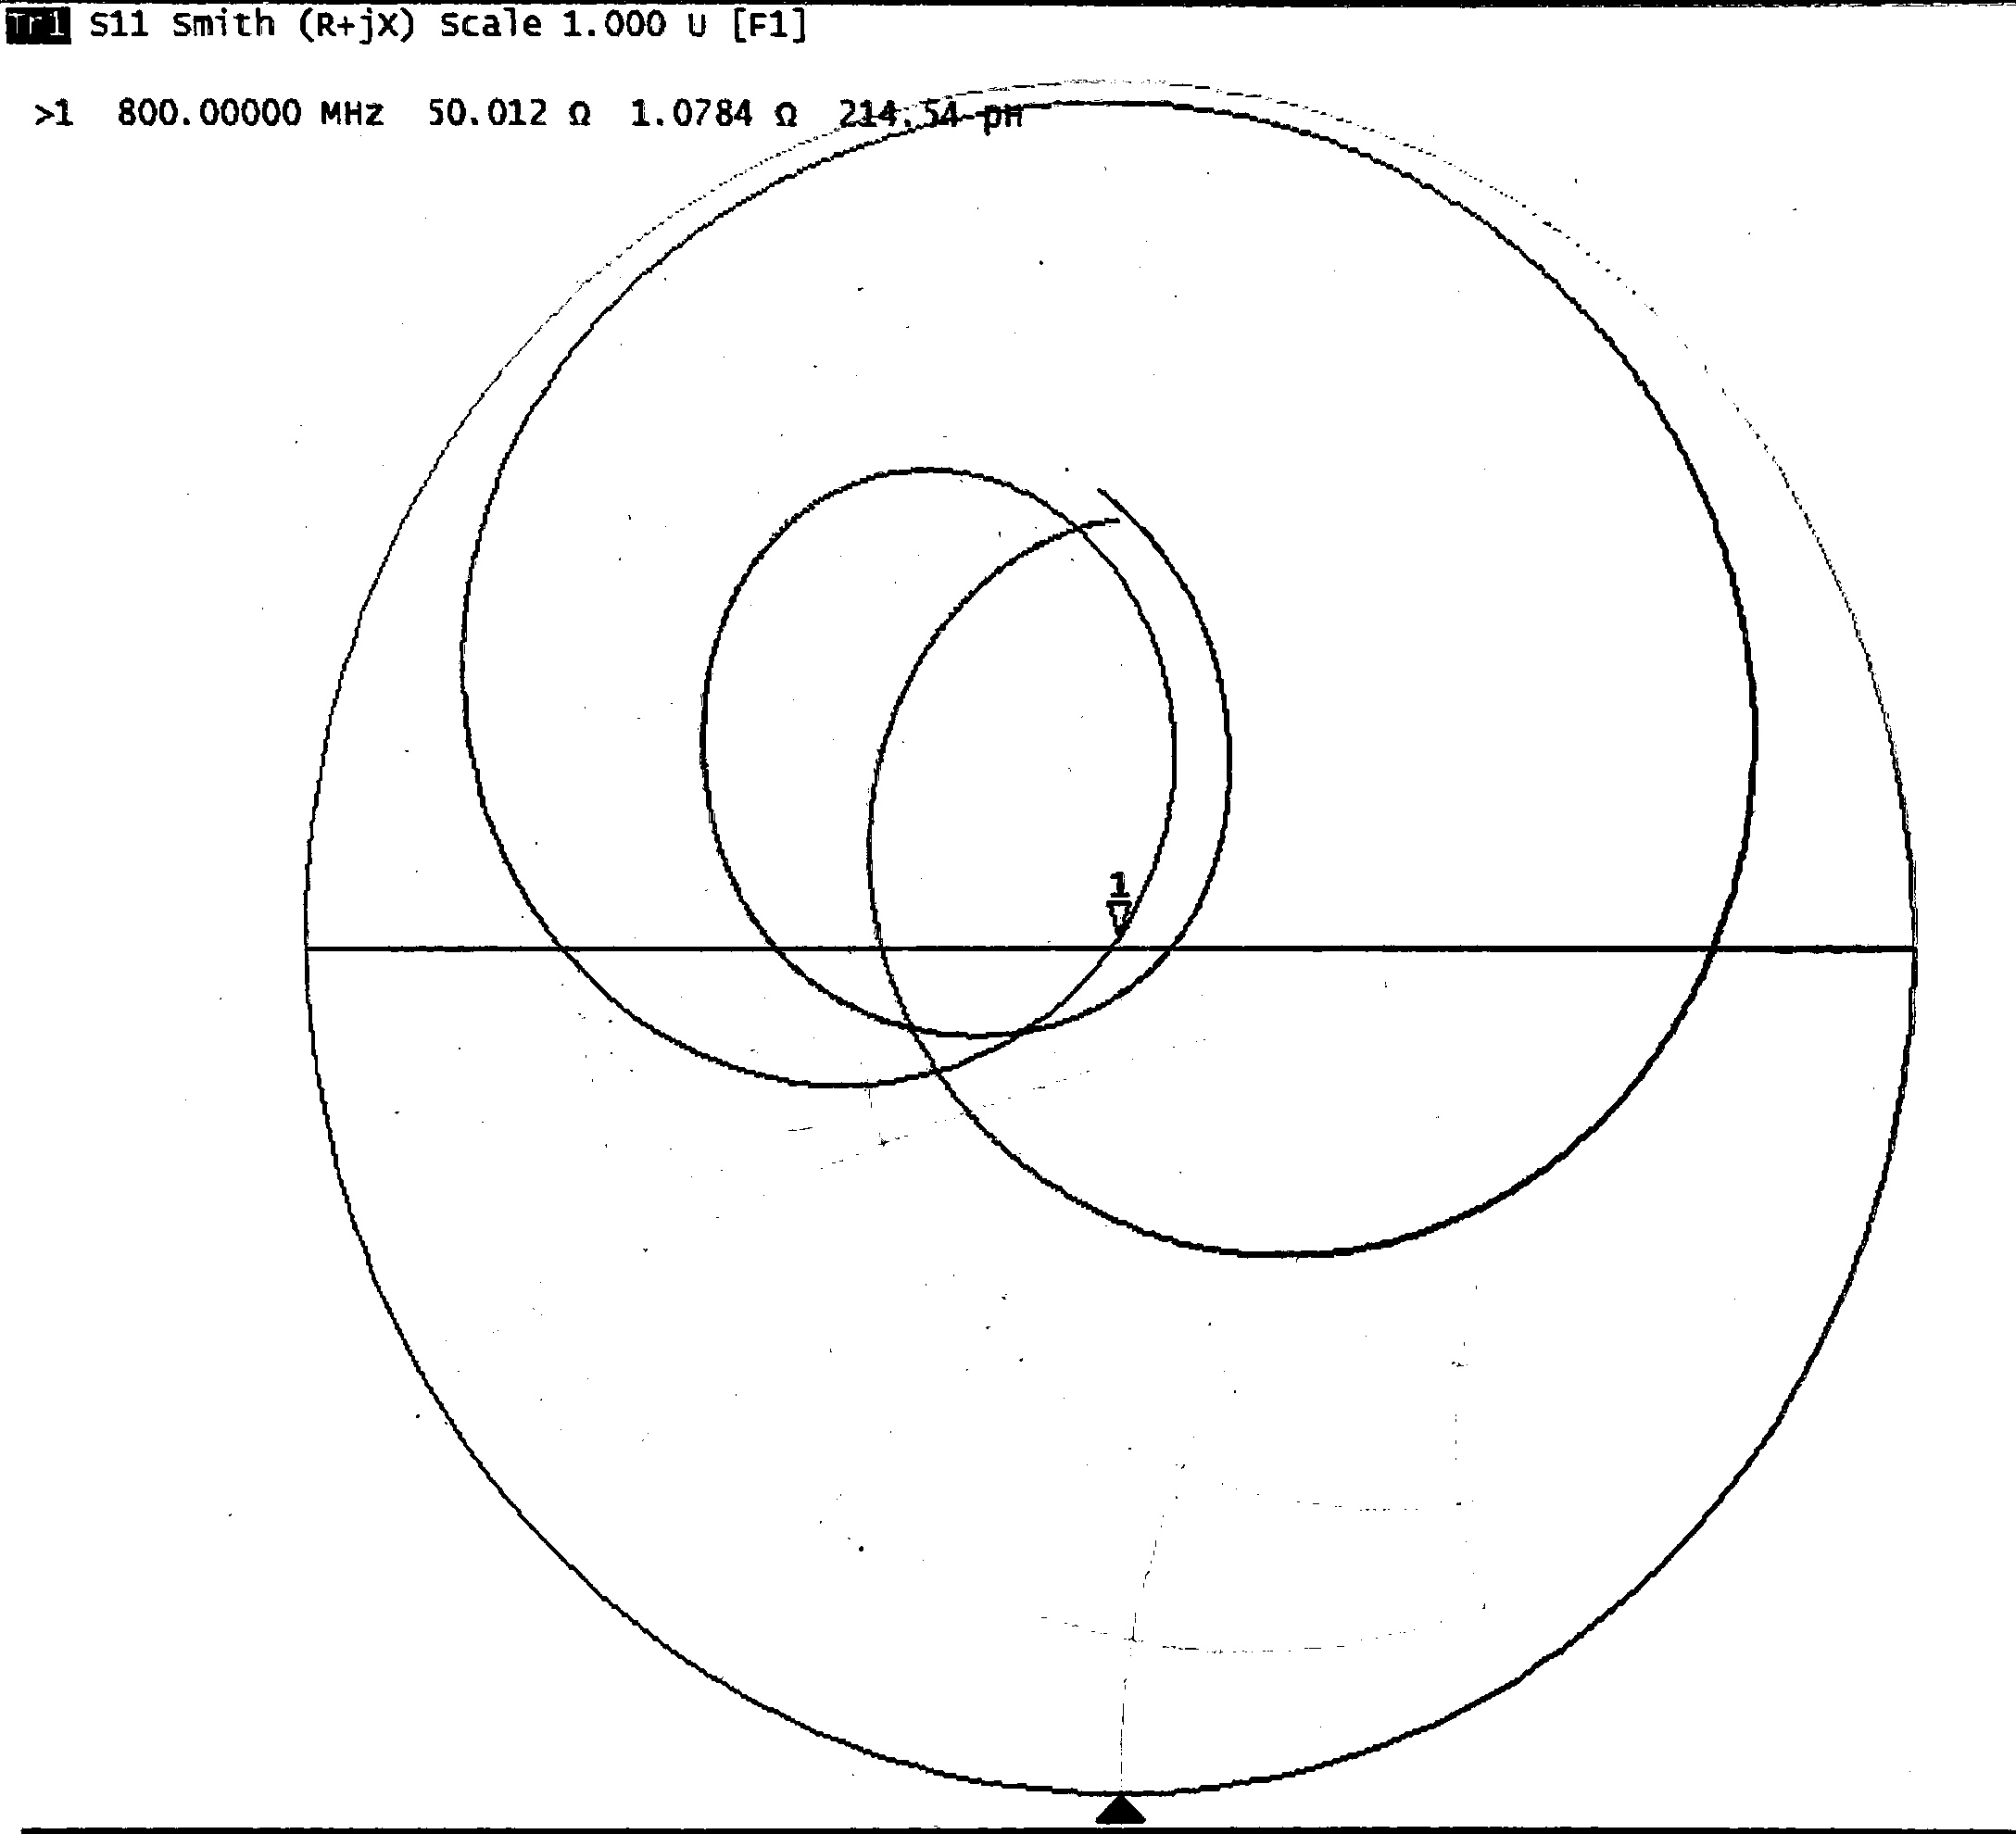
\includegraphics[width=\textwidth]{../photos/lab3/matching_long_pair.jpg}
    \caption{Matched load using the longer length stubs}
  \end{subfigure}
  \caption{Measuring input impedance over our frequency range for short and long stub length solutions\vspace{-0.3cm}}
  \label{matched_stubs}
\end{figure}

\section{The Standing Wave Ratio and Bandwidth Calculations}

Since the input impedenace of the matching network changes with frequency, it is important to see the signal transfer
characteristics of the matching network to determine the bandwidth of frequencies that "pass" over to the load without 
much distortion and reduction in amplitude. We use the voltage standing wave ratio ($\text{VSWR}$) to define bandwidth, 
$\text{BW}$, as,
\[
  \text{VSWR}(\omega) = \frac{1+||\Gamma_L(\omega)||}{1-||\Gamma_L(\omega)||} \quad \text{and} \quad \text{BW} = 
  \left\{\omega \in \mathbb{R}^{+} \middle | \text{VSWR}(\omega) \leq 2\right\}
\]
Here we note that the time-averaged power transmitted to load is given by $\langle P \rangle = \frac{||V_0^+||^2}{2Z_0}(1-||\Gamma_L||^2) = \langle P_\text{max} \rangle\cdot(1-||\Gamma_L||^2)$,
where $\langle P_\text{max}\rangle$ is the maximum time-averaged power that can be delivered to the load which happens for a matched load when $\Gamma_L = 0$.
At $\text{VSWR} = 2, \Gamma_L = \frac{1}{3} \implies \langle P \rangle \approx 0.89\cdot \langle P_\text{max}\rangle$, and thus our definition considers 
bandwith to be the range of frequencies where the power is delivered to the load at approximately $90\%$ efficiency. Also note 
that at bandwidth limiting frequencies, $20\log(\Gamma_L) = \Gamma_\text{L, dB} \approx -10\text{ dB}$, which suggests that 
$\Gamma_L \geq -10\text{ dB}$ are acceptable values for the refelection coefficient such that the delivered signal's power is not 
degraded as much. We have also recorded the VSWR versus frequency plots on the VNA for both fundamental solutions, shown in Figure 4, and the 
bandwidths can be found in Table 4.

\begin{table}[h]
  \[
    \begin{array}{c|c}
        \textbf{Stub Pair} & \textbf{Bandwidth in} \text{ MHz}\\ \hline
        \text{Short} &  [692, 908]\\
        \text{Long} & [788, 808]\vspace{-0.25cm}
    \end{array}
\]
\caption{Bandwidth of the short and long matching networks}
\end{table}

We note that shorter stubs give better performance in terms of bandwidth since they have less variation of electrical parameters,
specifcially input impedance, with frequency compared to the longer stubs. This is beacuse the normalized input admittance of short circuited
stubs is $Y_\text{in,N}=-j\cot(\beta L)$, where $\beta = \omega\sqrt{L'C'}$, where $L$ is the length of the stub and $L',C'$ are 
distributed inductance and capacitance of the stub, respectively. Thus, for a fixed frequency, $\omega$, if $L$ is increased, $Y_\text{in,N}$
and $\Gamma_L$ will vary faster, which can also be seen in Figure 3. As a result, for longer stubs we get a smaller window 
of frequencies we can use to fit the bandwidth constraint, whereas for shorter stubs the bandwidth is larger.

\begin{figure}[ht]
  \centering
  \begin{subfigure}[b]{0.45\textwidth}
      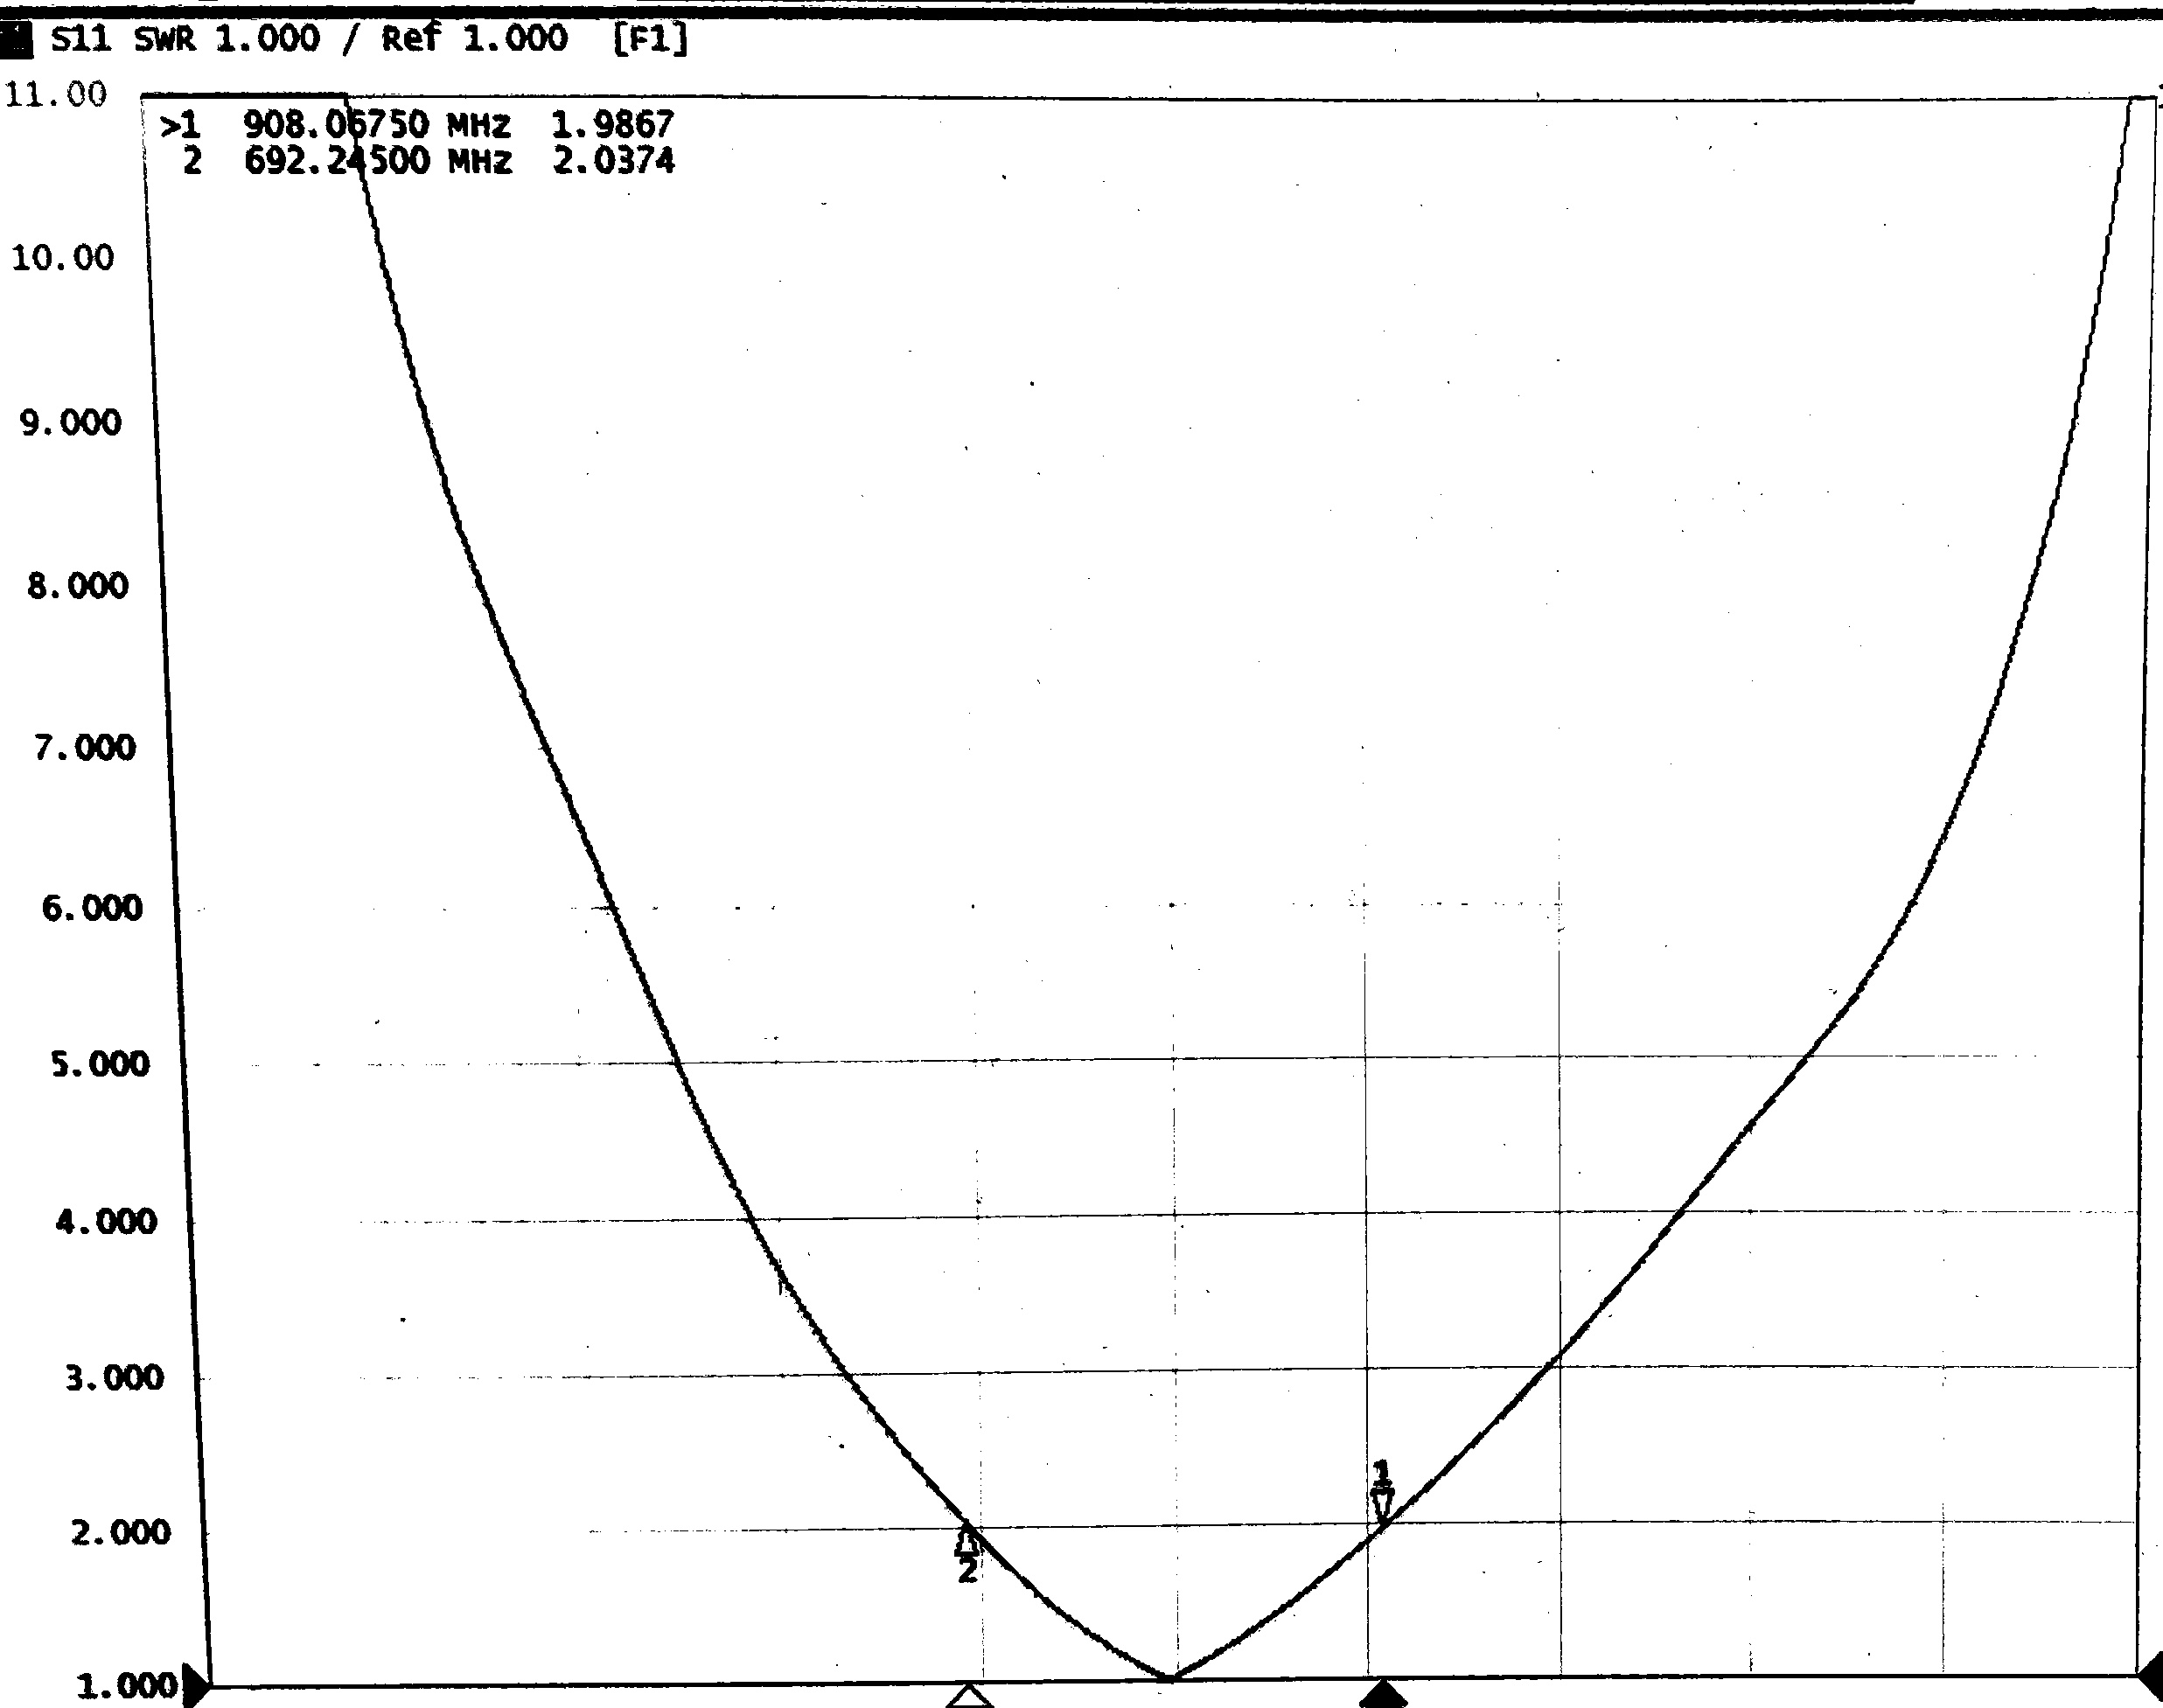
\includegraphics[width=\textwidth]{../photos/lab3/short_pair_bw.jpg}
      \caption{VSWR vs frequency for the shorter length stubs}
  \end{subfigure}
  \quad
  \begin{subfigure}[b]{0.45\textwidth}
    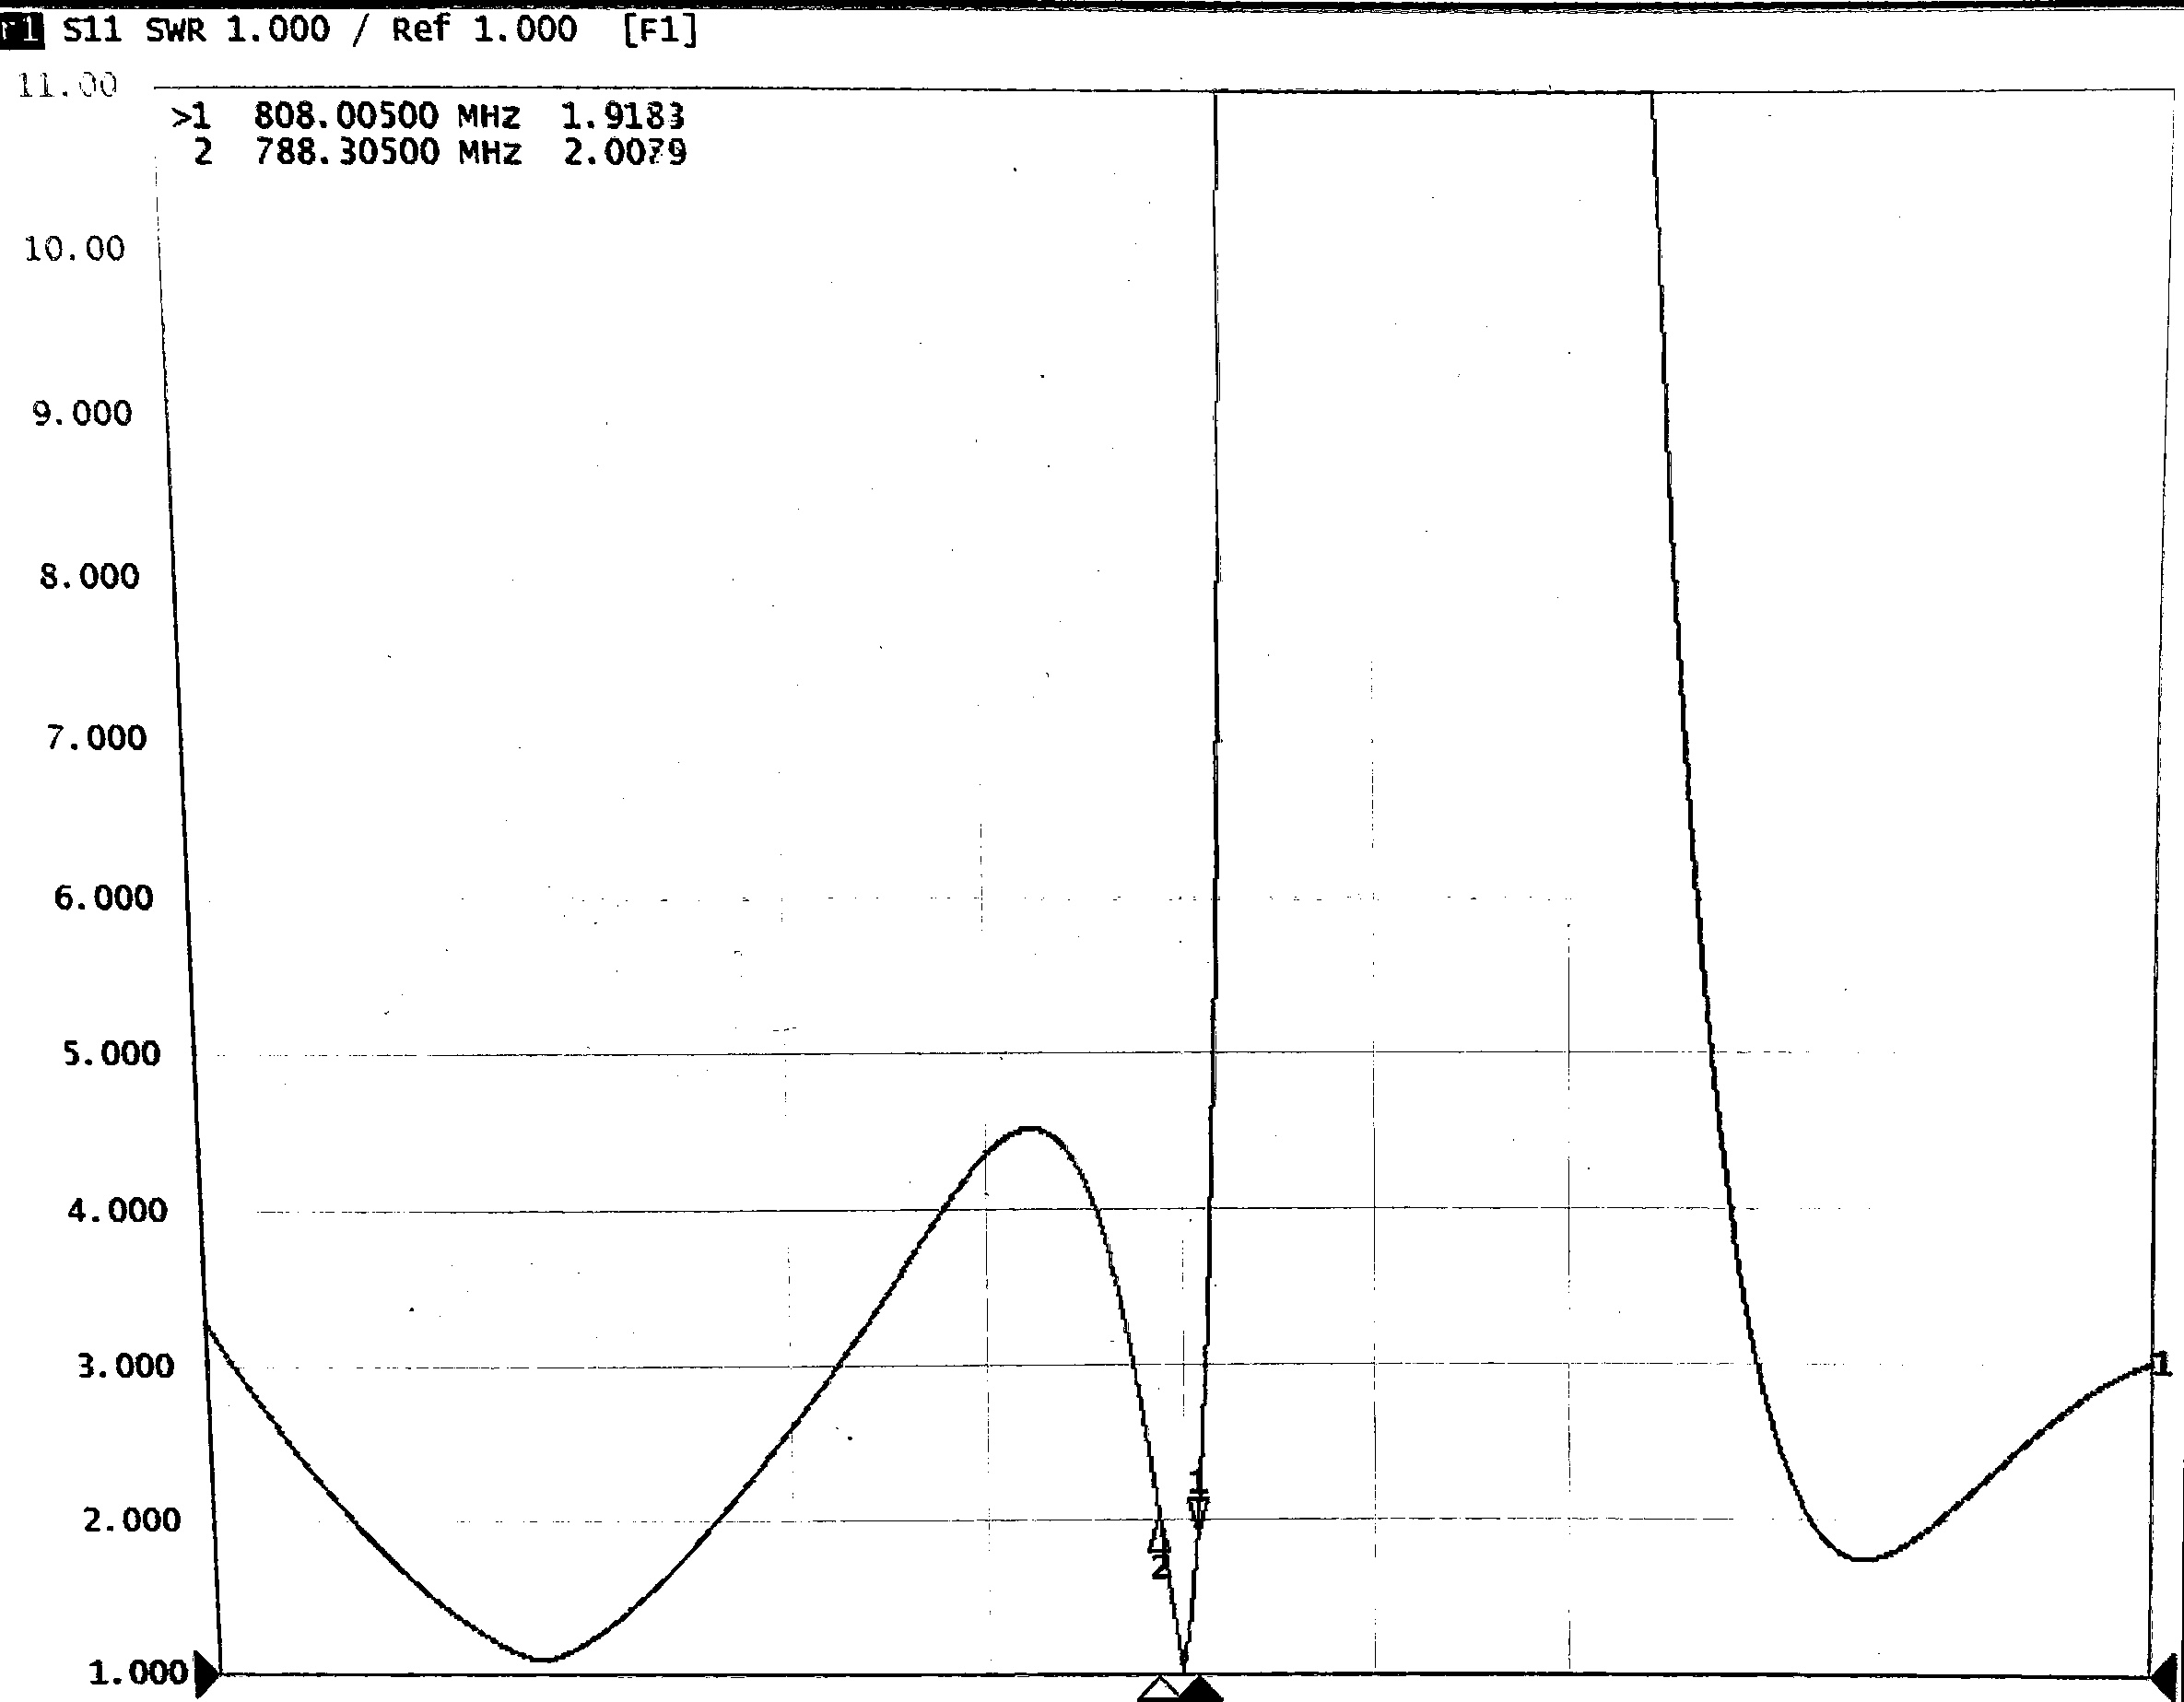
\includegraphics[width=\textwidth]{../photos/lab3/long_pair_bw.jpg}
    \caption{VSWR vs frequency for the longer length stubs}
  \end{subfigure}
  \caption{Variation of VSWR over our frequency range\vspace{-0.3cm}}
  \label{vswr_freq}
\end{figure}

\section{Notes}

All images taken during the lab were post-processed in a batch using a custom script
that bit-wise inverts the pixels and binarizes the resulting image based on a custom threshold.
No adjustments or modifications were made to the readings, for which the measurements on the VNA
are also shown alongside the waveforms. All scripts and related work can be found at 
\href{https://github.com/pranshumalik14/ece320-labs}{\texttt{github.com/pranshumalik14/ece320-labs}}.

\end{document}